\documentclass{article}

% Packages
\usepackage{fancyhdr}
\usepackage{graphicx}
\usepackage{amsmath}
\usepackage{biblatex}
\usepackage{pgfgantt}
\usepackage{float}
\usepackage[table, xcdraw]{xcolor}

\addbibresource{bib.bib}

% Simple multiline comment
\newcommand{\mycomment}[1]{}

% Configuring Fancy hdr
\pagestyle{fancy}

\fancyhead[R]{Project Formulation}
\fancyhead[L]{Philip Oliver Mejer Jørgensen}

% Configuring title page
\title{Detection of Vinyl Chloride in environmental water samples}
\author{Project Formulation\\Philip Oliver Mejer Jørgensen}
\date{Fall 2023}

% Main document
\begin{document}
\maketitle

\section*{Background}
Humans produce waste, whether that is as an individual or on an industrial level. A lot of the waste that is being produced, end up in our water supply contaminating it.
An example of a toxic waste product that can end up in the water supply is vinyl chloride \textit{(VC)}, one of the primary areas VC is found is in the production of PVC.
PVC plastic is used as pipes for plumbing, bottles, and more\cite{pvc_applications}.
Vinyl chloride is a highly volatile compound which makes it both hard to detect, and making it more dangerous.
This has created a need for a fast and simple solution for detecting the concentration of vinyl chloride in water samples.

This has led the company Water Care Guard \textit{(WCG)} to develop an on-site lab kit that fits in a suitcase, which is able to test a water sample for the concentration of vinyl chloride amongst other substances.

This project is done in collaboration with Roana from SDU Nano Syd and Water Care Guard.

\vspace{15mm}

\section*{Problem}
As it stands at the moment, when you want to detect vinyl chloride in water samples you use a method of analysis called \textit{"Gas chromatographic (GC) analysis"}\cite{vc_who}.
Gas chromatographic analysis is an analysis method in which the sample is being heated to the point of each component in the sample is being vaporized, where it then enters a column where the different components are being separated, such that it can be detected.\cite{gc_shimadzu}
The process of sending a water sample to a laboratory and getting the measurements made, is time-consuming and expensive.
It can take up to two weeks to get a water sample analyzed in a laboratory.\cite{water_analysis_cwt}
The solution with Water Care Guard, aims to reduce this time, by creating an onsite \textit{laboratory kit}, where you can test the water sample.
It is using the fact that the refractive index of the solution with added enzyme is dependent on the concentration of vinyl chloride in the solution.
The refractive index can be determined using a spectrophotometer and a cuvette with a photonic crystal applied to one side.\cite{ri_dtu}\\

The main part of the project is going to be about building a database for different vinyl chloride concentrations and the refractive index shift for the corresponding vinyl chloride concentration.
In addition, the data from the database should be analyzed to be able to get a prediction for the concentration of vinyl chloride in the solution based on the sample given.\\

The second part of the project is building a simplified user interface for the suitcase, which could be installed on a tablet in the suitcase or another display that the user can interact with.
It could even be used on the smartphone of the user, or something else.
This could be accomplished by making a dedicated app, or by having a website that is hosted on a computer in the suitcase, this would allow the user to access the user interface from either a tablet in the suitcase or from their computer or smartphone.\\

\vspace{15mm}
\section*{Timetable and milestones}
The project is divided into 3 main parts:\\
\begin{itemize}
    \item Building the database
    \item Analyzing the data
    \item User interface
\end{itemize}

The different parts are going to overlap, but it is primarily going to be in the order of the first part is focusing on building the database then about finding a way to analyze the data, and lastly building the user interface.\\
The project is divided up with the intention of spending 8 hours per day, 5 days a week on the project i.e. 40 hours a week.

\subsection*{Gantt chart}
\begin{figure}[H]
\centering
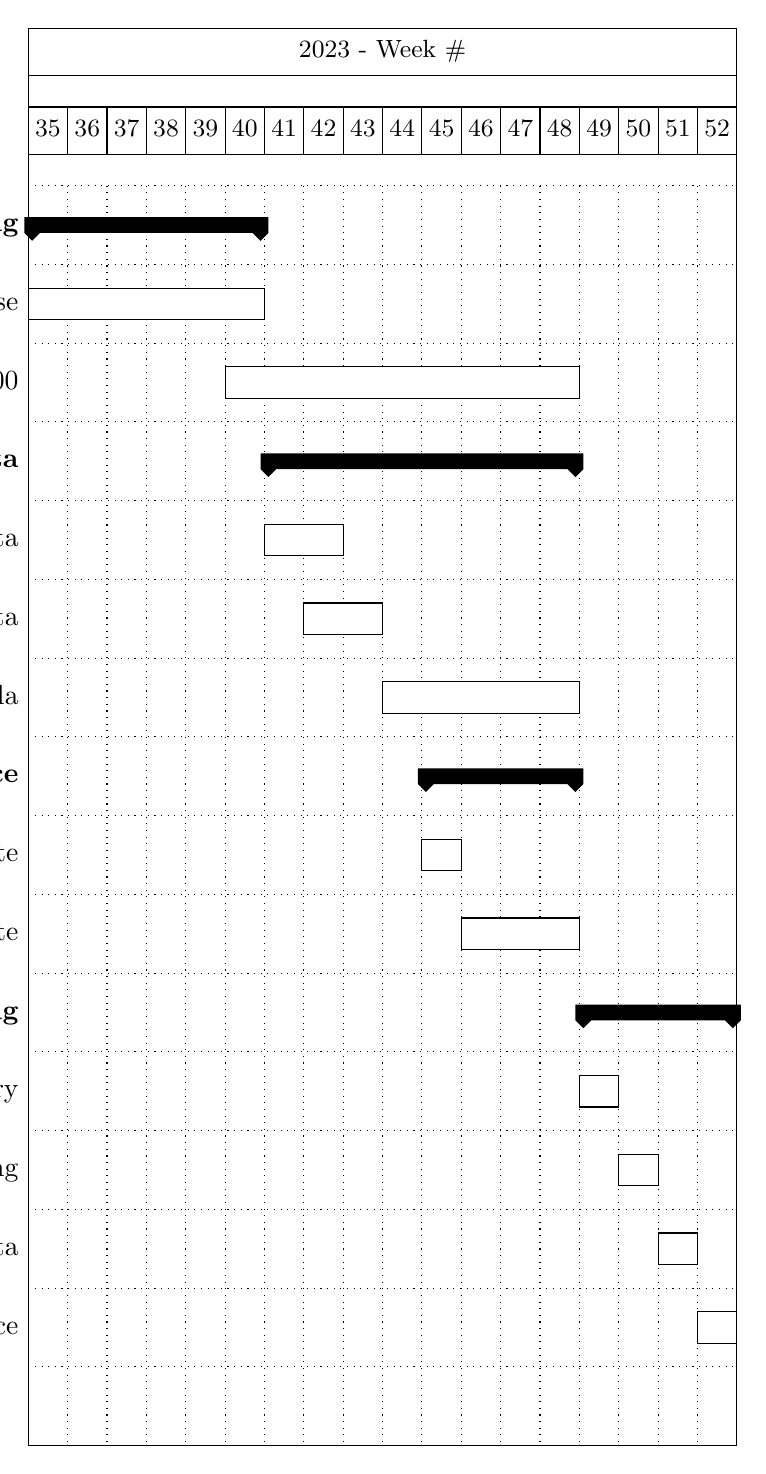
\begin{tikzpicture}
\begin{pgfinterruptboundingbox}
    \begin{ganttchart}[
        hgrid,
        vgrid,
        canvas/.append style={alias=frame}
    ]{35}{52}
    \gantttitle{2023 - Week \#}{18} \\
    \gantttitlelist{35,...,52}{1}\\
    \ganttgroup{Database building}{35}{40} \\
    \ganttbar{Using the WCG suitcase}{35}{40} \\
    \ganttbar{Using the Shimadzu UV-1900}{40}{48} \\

    \ganttgroup{Analyzing data}{41}{48} \\
    \ganttbar{Filter and process data}{41}{42} \\
    \ganttbar{Consolidating all data}{42}{43} \\
    \ganttbar{Create best fit formula}{44}{48} \\

    \ganttgroup{User interface}{45}{48} \\
    \ganttbar{Creating basic website}{45}{45} \\
    \ganttbar{Adding database to the website}{46}{48} \\

    \ganttgroup{Writing}{49}{52} \\
    \ganttbar{Background and theory}{49}{49} \\
    \ganttbar{Database building}{50}{50} \\
    \ganttbar{Analyzing data}{51}{51} \\
    \ganttbar{User interface}{52}{52} \\

    \end{ganttchart}
\end{pgfinterruptboundingbox}
\useasboundingbox (frame.south west) rectangle (frame.north east);
\end{tikzpicture}
\caption{The timetable in a Gantt chart format, divided up in weeks}
\label{timetable}
\end{figure}

\mycomment{
    What to include in the Gantt chart.
    Database building
    Analyzing data
    User interface
    Writing
        - The different sections of the project each gets a week

}

\vspace{15mm}
\section*{Risk assessment}

The primary risk associated with the project is regards to dealing with the chemicals in making the measurements.

\begin{table}[H]
\resizebox{\textwidth}{!}{%
\begin{tabular}{|l|l|l|l|}
\hline
\rowcolor[HTML]{C1DBFF} 
\textbf{Issue}                                                                                                         & \textbf{Who  is involved}                                                      & \textbf{Impact/Probability} & \textbf{Mitigative actions}                                                                              \\ \hline
\rowcolor[HTML]{FFCCC9} 
\begin{tabular}[c]{@{}l@{}}High volatility and\\ toxicity of Vinyl Chloride.\\ Working with the chemicals\end{tabular} & \begin{tabular}[c]{@{}l@{}}Operator performing\\ the measurements\end{tabular} & High/High                   & \begin{tabular}[c]{@{}l@{}}Using:\\ - labcoat\\ - safety glasses\\ - working in a fume hood\end{tabular} \\ \hline
\end{tabular}%
}
\caption{The risk assessment table}
\label{risk-table}
\end{table}

\vspace{15mm}
\printbibliography
\end{document}